\documentclass[10pt, a4paper]{article}

\usepackage{ctex}
\usepackage{xeCJK}
\usepackage{caption}
\usepackage{geometry}
\geometry{
    left = 0.6in,
    right = 0.6in,
    top = 0.8in,
    bottom = .6in
}
\usepackage{amssymb}
\usepackage{amsbsy}
\usepackage{amsmath}
\usepackage{xcolor}
\usepackage{mathrsfs}
\usepackage{graphicx}
\usepackage{pifont}
\usepackage{tikz}
\usepackage{tasks}
\settasks{
    label = \textcolor{purple}{\Alph*.},
    label-width = 14pt
}
\pagestyle{empty}

\newcommand{\Title}[3]{
    \begin{center}
        \Large \textbf{中国电子学会 #1~年~#2~月 Scratch~#3级考试}
    \end{center}
}
\newcommand{\TimeAndName}[1]{
    \begin{center}
        考试时间:~#1~ 分钟 \qquad\qquad\qquad\qquad 姓名:\underline{\quad\quad\quad\quad}
    \end{center}
}
\newcommand{\hq}{\hfill(\qquad)}

\begin{document}
    \Title{2023}{05}{二} % 标题
    \TimeAndName{60} % 考试时间及姓名

    % 单选题
    \vspace{2mm}
    {\noindent\textbf{第一部分、单选题(共 25 题,每题 2 分,共50分.)}}
    \begin{enumerate}
        % 1
        \item 运行下列哪段程序,可以让狗狗走到木屋门口? \hq
        
        \begin{minipage}{.2\textwidth}
            \centering
            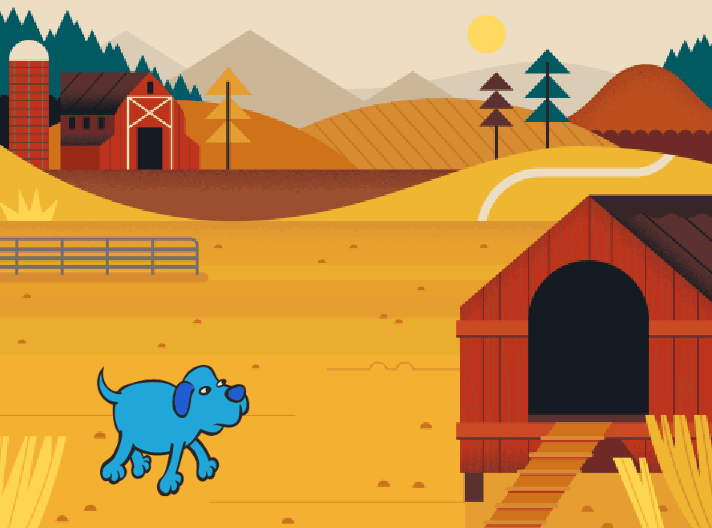
\includegraphics[width=.9\textwidth]{figure/1.png}
        \end{minipage}
        \begin{minipage}{.7\textwidth}
            \begin{tasks}(4)
                \task 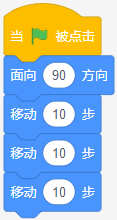
\includegraphics[width=.1\textwidth]{figure/1a.png}
                \task 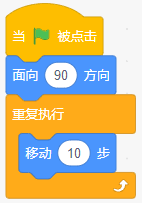
\includegraphics[width=.13\textwidth]{figure/1b.png}
                \task 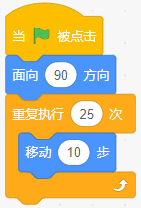
\includegraphics[width=.13\textwidth]{figure/1c.png}
                \task 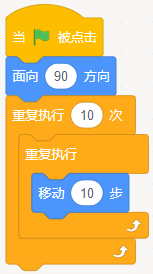
\includegraphics[width=.11\textwidth]{figure/1d.png}
            \end{tasks}
        \end{minipage}

        % 2
        \item 下列哪个选项可以控制:按下左键扫帚向左旋转15度,按下右键扫帚向右旋转15度?\hq
        
        \begin{minipage}{.15\textwidth}
            \centering
            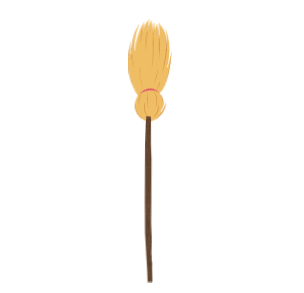
\includegraphics[width=\textwidth]{figure/2.png}
        \end{minipage}
        \begin{minipage}{.75\textwidth}
            \begin{tasks}(4)
                \task 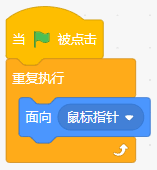
\includegraphics[width=.17\textwidth]{figure/2a.png}
                \task 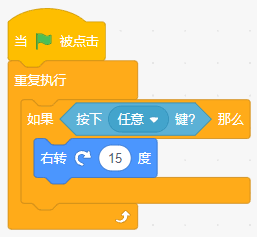
\includegraphics[width=.18\textwidth]{figure/2b.png}
                \task 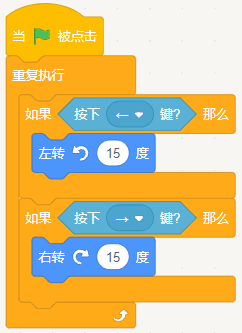
\includegraphics[width=.15\textwidth]{figure/2c.png}
                \task 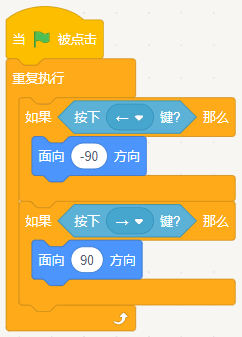
\includegraphics[width=.15\textwidth]{figure/2d.png}
            \end{tasks}
        \end{minipage}

        % 3
        \item 下列哪个选项可以把音波曲线图变成一条直线? \hq
        \begin{tasks}(4)
            \task 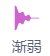
\includegraphics[width=.05\textwidth]{figure/3a.png}
            \task 
\includegraphics[width=.05\textwidth]{figure/3b.png}
            \task 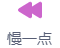
\includegraphics[width=.05\textwidth]{figure/3c.png}
            \task 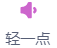
\includegraphics[width=.05\textwidth]{figure/3d.png}
        \end{tasks}

        % 4
        \item 下图的六芒星一共包含多少个三角形?\hq
        \begin{tasks}(4)
            \task 2
            \task 8
            \task 26
            \task 10
        \end{tasks}

        \begin{figure}[htbp]
            \centering
            \begin{minipage}[t]{.35\textwidth}
                \centering
                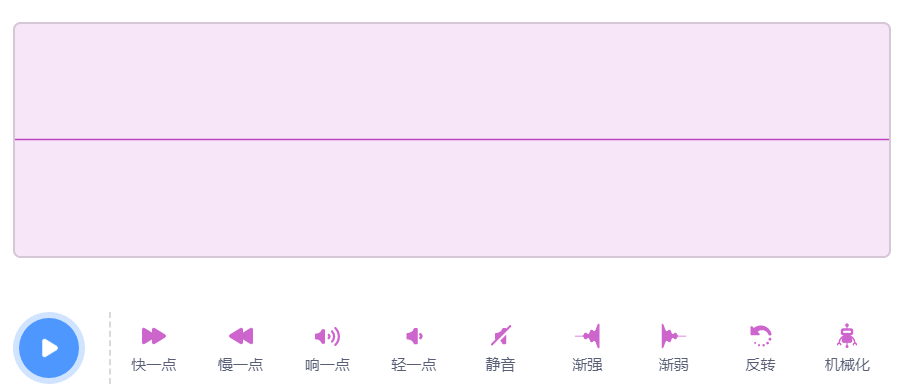
\includegraphics[width=\textwidth]{figure/3.png}
                \caption*{第 3 题}
            \end{minipage}
            \begin{minipage}[t]{.2\textwidth}
                \centering
                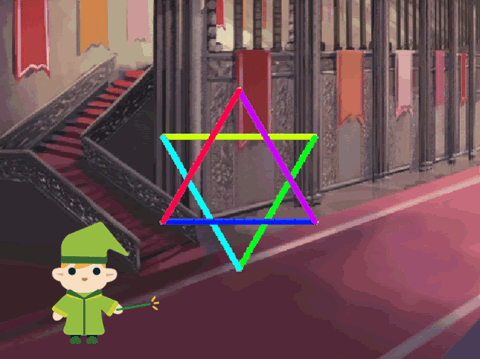
\includegraphics[width=\textwidth]{figure/4.png}
                \caption*{第 4 题}
            \end{minipage}
            \begin{minipage}[t]{.3\textwidth}
                \centering
                \begin{minipage}[t]{.55\textwidth}
                    \centering
                    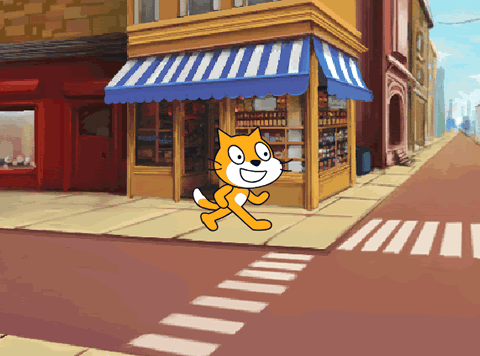
\includegraphics[width=\textwidth]{figure/6-1.png}
                \end{minipage}
                \begin{minipage}[t]{.4\textwidth}
                    \centering
                    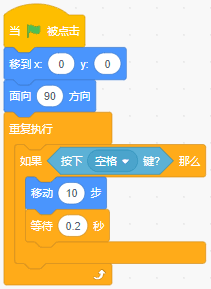
\includegraphics[width=\textwidth]{figure/6-2.png}
                \end{minipage}
                \caption*{第 6 题}
            \end{minipage}
        \end{figure}

        % 5
        \item 观察数列规律:1, 1, 2, 3, 5, 8, (\qquad),请问括号里应该填写? \hq
        \begin{tasks}(4)
            \task 10
            \task 13
            \task 14
            \task 15
        \end{tasks}

        % 6
        \item 小猫的程序如下图所示,点击绿旗,按下1次空格键后,小猫的坐标为?\hq
        \begin{tasks}(4)
            \task $(10, 0)$
            \task $(0, 10)$
            \task $(0, 0)$
            \task $(10, 10)$
        \end{tasks}

        % 7
        \item 点击绿旗,运行如右图所示的程序,程序中的蓝色跟舞台上的蓝色一致,下列选项描述正确的是?\hq

        \begin{minipage}{.22\textwidth}
            \centering
            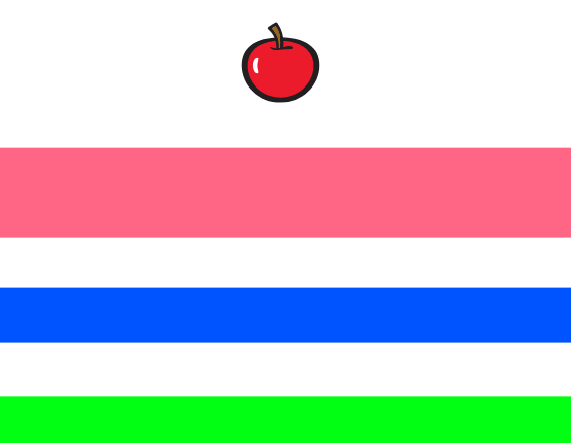
\includegraphics[width=\textwidth]{figure/7-1.png}
        \end{minipage}
        \begin{minipage}{.17\textwidth}
            \centering
            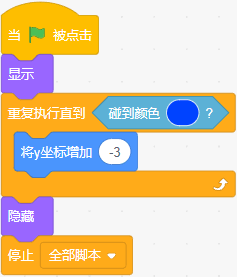
\includegraphics[width=\textwidth]{figure/7-2.png}
        \end{minipage}
        \begin{minipage}{.5\textwidth}
            \centering
            \begin{tasks}
                \task 苹果往下落,当碰到了蓝色时就不见了
                \task 苹果往下落,当碰到了绿色时就不见了
                \task 苹果往下落,当碰到了红色时就不见了
                \task 苹果一直往下落,不会隐藏
            \end{tasks}
        \end{minipage}

        \newpage
        % 8
        \item 小明数学考了88分,语文比数学多考了2分,英语比语文少考了5分,请问小明英语考了多少分?\hq
        \begin{tasks}(4)
            \task 88分
            \task 90分
            \task 85分
            \task 83分
        \end{tasks}

        % 9
        \item 根据以下规律,请问位置7上应该放置什么图形?\hq
        
        \begin{minipage}{.3\textwidth}
            \centering
            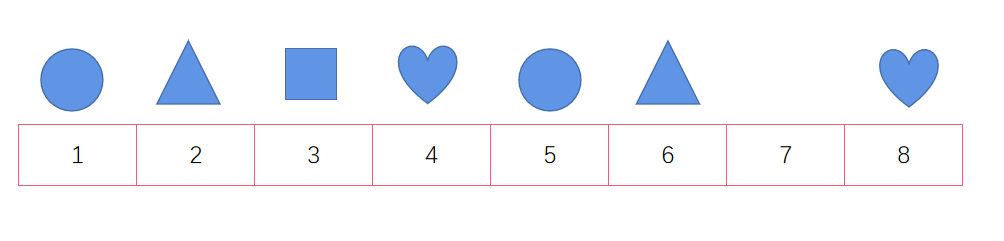
\includegraphics[width=\textwidth]{figure/9.png}
        \end{minipage}
        \begin{minipage}{.6\textwidth}
            \begin{tasks}(4)
                \task 
\includegraphics[width=.05\textwidth]{figure/9a.png}
                \task 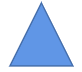
\includegraphics[width=.05\textwidth]{figure/9b.png}
                \task 
\includegraphics[width=.05\textwidth]{figure/9c.png}
                \task 
\includegraphics[width=.05\textwidth]{figure/9d.png}
            \end{tasks}
        \end{minipage}

        % 10
        \item 现有“车”和“车位”两个角色,角色初始位置如下图所示,运行一次程序,模拟倒车入库的过程,那么 \ding{172} 处应填写?\hq
        \begin{tasks}(4)
            \task 
\includegraphics[width=.1\textwidth]{figure/10a.png}
            \task 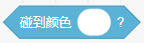
\includegraphics[width=.1\textwidth]{figure/10b.png}
            \task 
\includegraphics[width=.12\textwidth]{figure/10c.png}
            \task 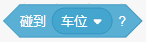
\includegraphics[width=.1\textwidth]{figure/10d.png}
        \end{tasks}

        % 11
        \item 点击绿旗,运行下列程序后,角色说出的值是?\hq
        \begin{tasks}(4)
            \task $a$ 和 $p$
            \task $ab$
            \task $3.33$
            \task $3$
        \end{tasks}

        \begin{figure}[htbp]
            \centering
            \begin{minipage}[t]{.28\textwidth}
                \centering
                \begin{minipage}[t]{.5\textwidth}
                    \centering
                    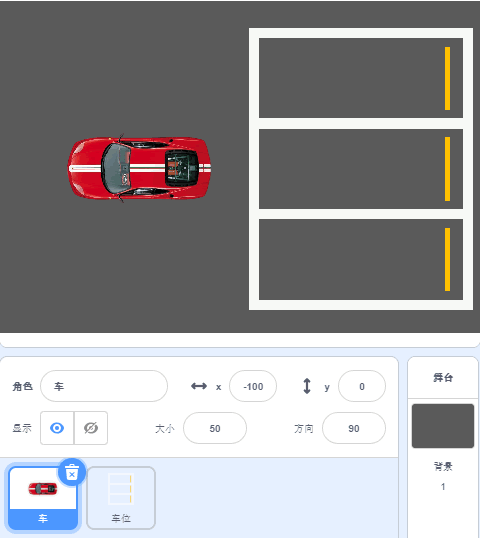
\includegraphics[width=\textwidth]{figure/10-1.png}
                \end{minipage}
                \begin{minipage}[t]{.4\textwidth}
                    \centering
                    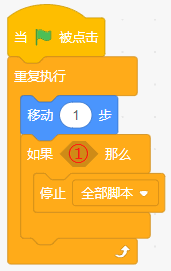
\includegraphics[width=\textwidth]{figure/10-2.png}
                \end{minipage}
                \caption*{第 10 题}
            \end{minipage}
            \begin{minipage}[t]{.26\textwidth}
                \centering
                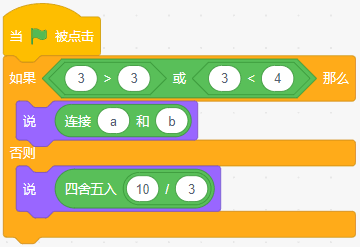
\includegraphics[width=\textwidth]{figure/11.png}
                \caption*{第 11 题}
            \end{minipage}
            \begin{minipage}[t]{.3\textwidth}
                \centering
                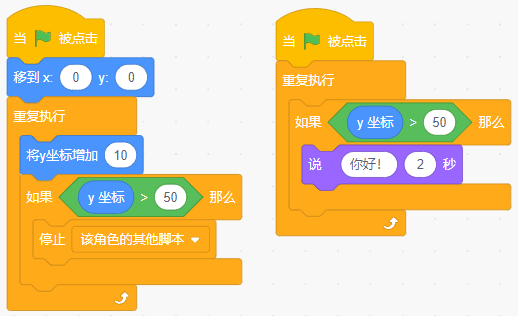
\includegraphics[width=\textwidth]{figure/13.png}
                \caption*{第 13 题}
            \end{minipage}
        \end{figure}

        % 12
        \item 声音编辑器中,对声音的调整不包含下列哪个选项?\hq
        \begin{tasks}(4)
            \task 响一点
            \task 快一点
            \task 渐强
            \task 重音
        \end{tasks}

        % 13
        \item 程序如上图所示,点击绿旗,运行程序后,下列选项描述正确的是?\hq
        \begin{tasks}
            \task 角色移动到 $(0,50)$ 处,说“你好!”2秒,继续移动到 $(0,60)$ 处停止
            \task 角色移动到 $(0,60)$ 处,说“你好!”2秒,然后停止
            \task 角色移动到屏幕顶端,中途在某个位置会说“你好!”2秒
            \task 角色移动到屏幕顶端,移动过程中未说出任何内容
        \end{tasks}
        
        % 14
        \item 下列哪个选项,可以让狐狸移到鹦鹉旁边?\hq
        
        \begin{minipage}{.2\textwidth}
            \centering
            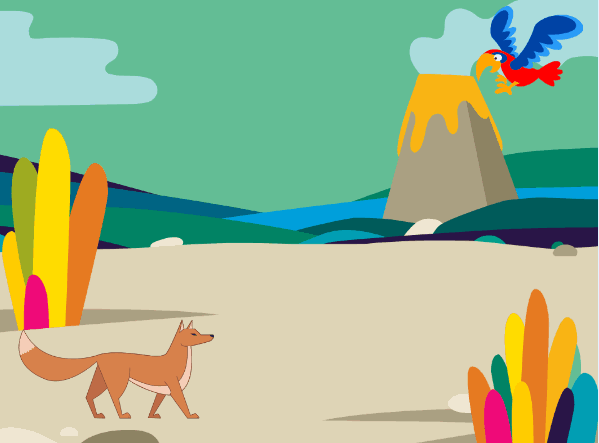
\includegraphics[width=\textwidth]{figure/14.png}
        \end{minipage}
        \begin{minipage}{.7\textwidth}
            \begin{tasks}(2)
                \task 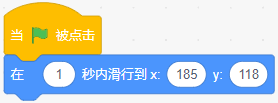
\includegraphics[width=.25\textwidth]{figure/14a.png}
                \task 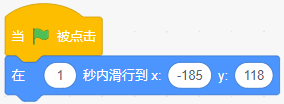
\includegraphics[width=.25\textwidth]{figure/14b.png}
                \task 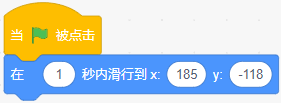
\includegraphics[width=.25\textwidth]{figure/14c.png}
                \task 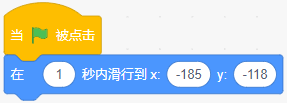
\includegraphics[width=.25\textwidth]{figure/14d.png}
            \end{tasks}
        \end{minipage}

        % 15
        \item 下列哪个选项实现的功能与下图程序一样?\hq
        
        \begin{minipage}{.13\textwidth}
            \centering
            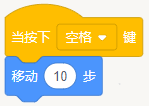
\includegraphics[width=\textwidth]{figure/15.png}
        \end{minipage}
        \begin{minipage}{.8\textwidth}
            \begin{tasks}(4)
                \task 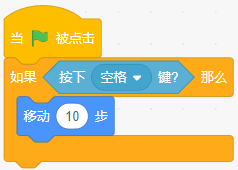
\includegraphics[width=.18\textwidth]{figure/15a.png}
                \task 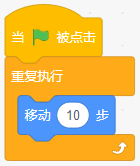
\includegraphics[width=.13\textwidth]{figure/15b.png}
                \task 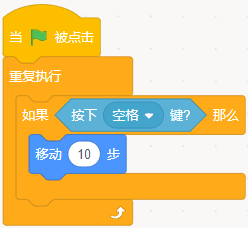
\includegraphics[width=.16\textwidth]{figure/15c.png}
                \task 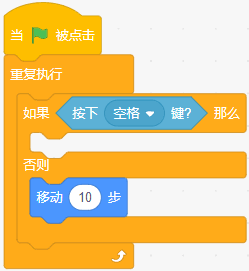
\includegraphics[width=.14\textwidth]{figure/15d.png}
            \end{tasks}
        \end{minipage}

        \newpage
        % 16
        \item 下列哪个选项的运算结果是true?\hq
        \begin{tasks}(4)
            \task 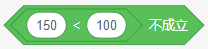
\includegraphics[width=.14\textwidth]{figure/16a.png}
            \task 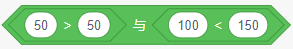
\includegraphics[width=.18\textwidth]{figure/16b.png}
            \task 
\includegraphics[width=.1\textwidth]{figure/16c.png}
            \task 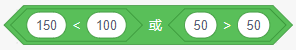
\includegraphics[width=.18\textwidth]{figure/16d.png}
        \end{tasks}

        % 17
        \item 默认小猫角色,运行下列程序,几秒钟以后小猫会完全消失?\hq
        \begin{tasks}(4)
            \task 9
            \task 10
            \task 6
            \task 5
        \end{tasks}

        % 18
        \item 舞台如下图所示,运行程序后,角色小猫最终会停留在哪个位置?\hq
        \begin{tasks}(4)
            \task 左上角
            \task 左下角
            \task 右上角
            \task 右下角
        \end{tasks}

        \begin{figure}[htbp]
            \centering
            \begin{minipage}[t]{.15\textwidth}
                \centering
                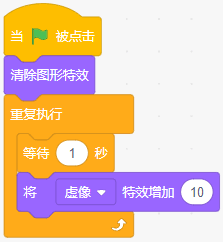
\includegraphics[width=\textwidth]{figure/17.png}
                \caption*{第 17 题}
            \end{minipage}
            \begin{minipage}[t]{.4\textwidth}
                \centering
                \begin{minipage}[t]{.5\textwidth}
                    \centering
                    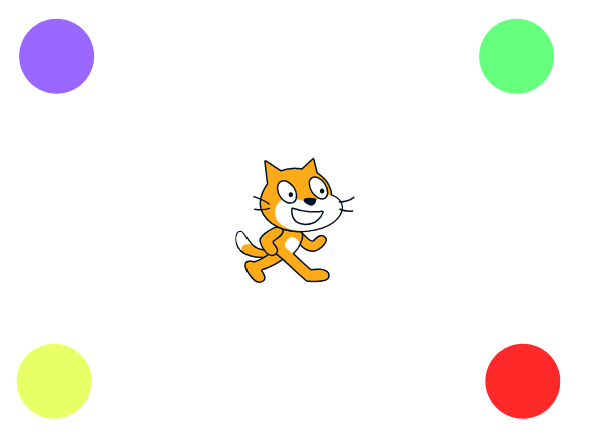
\includegraphics[width=\textwidth]{figure/18-1.png}
                \end{minipage}
                \begin{minipage}[t]{.4\textwidth}
                    \centering
                    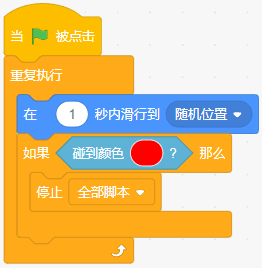
\includegraphics[width=\textwidth]{figure/18-2.png}
                \end{minipage}
                \caption*{第 18 题}
            \end{minipage}
            \begin{minipage}[t]{.1\textwidth}
                \centering
                \includegraphics[width=\textwidth]{figure/19.png}
                \caption*{第 19 题}
            \end{minipage}
            \begin{minipage}[t]{.12\textwidth}
                \centering
                \includegraphics[width=\textwidth]{figure/20.png}
                \caption*{第 20 题}
            \end{minipage}
            \begin{minipage}[t]{.2\textwidth}
                \centering
                \includegraphics[width=\textwidth]{figure/21.png}
                \caption*{第 21 题}
            \end{minipage}
        \end{figure}

        % 19
        \item 下列哪个选项可以绘制出上图所示图形?\hq
        \begin{tasks}(4)
            \task \includegraphics[width=.11\textwidth]{figure/19a.png}
            \task \includegraphics[width=.1\textwidth]{figure/19b.png}
            \task \includegraphics[width=.1\textwidth]{figure/19c.png}
            \task \includegraphics[width=.11\textwidth]{figure/19d.png}
        \end{tasks}

        % 20
        \item 运行上图程序后,舞台上出现的图形是?\hq
        \begin{tasks}(4)
            \task \includegraphics[width=.12\textwidth]{figure/20a.png}
            \task \includegraphics[width=.12\textwidth]{figure/20b.png}
            \task \includegraphics[width=.12\textwidth]{figure/20c.png}
            \task \includegraphics[width=.03\textwidth]{figure/20d.png}
        \end{tasks}

        % 21
        \item 下列哪个选项可以让小猫显示在大象和狮子的最前面?\hq
        \begin{tasks}(2)
            \task 将小猫“移到最前面”
            \task 将小猫“移到最后面”
            \task 将狮子“移到最后面”
            \task 将狮子和大象都“移到最前面”
        \end{tasks}

        % 22
        \item 舞台上有三个角色,猴子的程序如下图所示,另外两个角色没有程序,点击绿旗,下列描述正确的是? \hq
        
        \begin{minipage}{.2\textwidth}
            \centering
            \includegraphics[width=\textwidth]{figure/22-1.png}
        \end{minipage}
        \begin{minipage}{.1\textwidth}
            \centering
            \includegraphics[width=\textwidth]{figure/22-2.png}
        \end{minipage}
        \begin{minipage}{.63\textwidth}
            \begin{tasks}
                \task 猴子随鼠标移动,可能会遮挡另外两个角色
                \task 猴子随鼠标移动,可能会被另外两个角色遮挡
                \task 猴子不随鼠标移动,更不会被遮挡
                \task 三个角色都随鼠标移动,猴子会遮挡另外两个角色
            \end{tasks}
        \end{minipage}

        % 23
        \item 如下图所示,运行程序后,小猫面朝左图中的哪个方向?\hq
        \begin{tasks}(4)
            \task 北
            \task 南
            \task 西
            \task 北
        \end{tasks}

        \begin{figure}[htbp]
            \centering
            \begin{minipage}[t]{.26\textwidth}
                \centering
                \begin{minipage}[t]{.45\textwidth}
                    \centering
                    \includegraphics[width=\textwidth]{figure/23-1.png}
                \end{minipage}
                \begin{minipage}[t]{.5\textwidth}
                    \centering
                    \includegraphics[width=\textwidth]{figure/23-2.png}
                \end{minipage}
                \caption*{第 23 题}
            \end{minipage}
            \begin{minipage}[t]{.26\textwidth}
                \centering
                \begin{minipage}[t]{.55\textwidth}
                    \centering
                    \includegraphics[width=\textwidth]{figure/24-1.png}
                \end{minipage}
                \begin{minipage}[t]{.4\textwidth}
                    \centering
                    \includegraphics[width=\textwidth]{figure/24-2.png}
                \end{minipage}
                \caption*{第 24 题}
            \end{minipage}
            \begin{minipage}[t]{.35\textwidth}
                \centering
                \begin{minipage}[t]{.6\textwidth}
                    \centering
                    \includegraphics[width=\textwidth]{figure/25-1.png}
                \end{minipage}
                \begin{minipage}[t]{.35\textwidth}
                    \centering
                    \includegraphics[width=\textwidth]{figure/25-2.png}
                \end{minipage}
                \caption*{第 25 题}
            \end{minipage}
        \end{figure}

        % 24
        \item 要画出如上所示的图形,程序空白处从上往下应填写?\hq
        \begin{tasks}(4)
            \task 3,3
            \task 6,6
            \task 3,6
            \task 3,9
        \end{tasks}

        % 25
        \item 小猫和小鸡的初始位置如上图所示,运行程序后,小猫马上说“我抓到你了!”,程序空白处应填写?\hq
        \begin{tasks}(4)
            \task \includegraphics[width=.13\textwidth]{figure/25a.png}
            \task \includegraphics[width=.12\textwidth]{figure/25b.png}
            \task \includegraphics[width=.13\textwidth]{figure/25c.png}
            \task \includegraphics[width=.12\textwidth]{figure/25d.png}
        \end{tasks}
    \end{enumerate}

    % 判断题
    {\noindent\textbf{第二部分、判断题(共 10 题,每题 2 分,共20分.)}}
    \begin{enumerate}
        \setcounter{enumi}{25}
        % 26
        \item 如下图所示,点击绿旗,运行程序后,舞台上会出现五个机器人。\hq

        % 27
        \item 如图\includegraphics[width=.15\textwidth]{figure/27.png}所示,可以把声音波形中选中的部分删除。\hq
        
        \begin{figure}[htbp]
            \centering
            \begin{minipage}[t]{.2\textwidth}
                \centering
                \begin{minipage}[t]{.5\textwidth}
                    \centering
                    \includegraphics[width=\textwidth]{figure/26-1.png}
                \end{minipage}
                \begin{minipage}[t]{.45\textwidth}
                    \centering
                    \includegraphics[width=\textwidth]{figure/26-2.png}
                \end{minipage}
                \caption*{第 26 题}
            \end{minipage}
            \begin{minipage}[t]{.35\textwidth}
                \centering
                \begin{minipage}[t]{.5\textwidth}
                    \centering
                    \includegraphics[width=\textwidth]{figure/29-1.png}
                \end{minipage}
                \begin{minipage}[t]{.45\textwidth}
                    \centering
                    \includegraphics[width=\textwidth]{figure/29-2.png}
                \end{minipage}
                \caption*{第 29 题}
            \end{minipage}
            \begin{minipage}[t]{.18\textwidth}
                \centering
                \includegraphics[width=\textwidth]{figure/30.png}
                \caption*{第 30 题}
            \end{minipage}
            \begin{minipage}[t]{.19\textwidth}
                \centering
                \includegraphics[width=\textwidth]{figure/31.png}
                \caption*{第 31 题}
            \end{minipage}
        \end{figure}

        % 28
        \item 积木\includegraphics[width=.1\textwidth]{figure/28.png}可以比较两个数字大小。\hq

        % 29
        \item 如上图所示,点击绿旗,运行程序后,小猫会一直在舞台来回移动,不会停止。\hq

        % 30
        \item 点击绿旗,运行上图程序后,小猫会说“我是大猫”。\hq

        % 31
        \item 运行下列程序,如果鼠标指针碰到角色,角色会隐藏。\hq

        \newpage
        % 32
        \item 小猫和老鼠的初始位置如下图所示,不断按下→键,小猫可以抓住老鼠。\hq

        % 33
        \item 气球程序如下图所示,运行下列程序后,气球能够上升并达到顶部后隐藏。\hq
        
        \begin{figure}[htbp]
            \centering
            \begin{minipage}[t]{.4\textwidth}
                \centering
                \begin{minipage}[t]{.5\textwidth}
                    \centering
                    \includegraphics[width=\textwidth]{figure/32-1.png}
                \end{minipage}
                \begin{minipage}[t]{.45\textwidth}
                    \centering
                    \includegraphics[width=\textwidth]{figure/32-2.png}
                \end{minipage}
                \caption*{第 32 题}
            \end{minipage}
            \begin{minipage}[t]{.17\textwidth}
                \centering
                \includegraphics[width=\textwidth]{figure/33.png}
                \caption*{第 33 题}
            \end{minipage}
            \begin{minipage}[t]{.14\textwidth}
                \centering
                \includegraphics[width=\textwidth]{figure/34.png}
                \caption*{第 34 题}
            \end{minipage}
            \begin{minipage}[t]{.25\textwidth}
                \centering
                \includegraphics[width=\textwidth]{figure/35.png}
                \caption*{第 35 题}
            \end{minipage}
        \end{figure}

        % 34
        \item 角色位于舞台的正中心,面向90方向,笔的颜色为蓝色,运行上图程序后,画出的轨迹是三角形。\hq

        % 35
        \item 小猫程序如上图所示,运行程序后,按下空格键,小猫静止不动。\hq
    \end{enumerate}

    {\noindent \textbf{第三部分、编程题(共 2 题,共30分.)}}
    \begin{enumerate}
        \setcounter{enumi}{35}
        
        % 36
        \item 接水果:
        
        1. 准备工作
        \begin{tasks}[label = (\arabic*)]
            \task 导入背景Blue Sky;
            \task 删除小猫角色,导入角色Bowl、Apple、Strawberry、Bananas。
        \end{tasks}
        2. 功能实现
        \begin{tasks}[label = (\arabic*)]
            \task 点击绿旗,角色Bowl、Apple、Strawberry、Bananas都设置好初始位置,Bowl在舞台下方,Apple、Strawberry、Bananas在舞台上方不同位置;
            \task 角色Bowl可以通过键盘左右键控制左右移动;
            \task 角色Apple、Strawberry、Bananas都可以从天上掉落下来;
            \task 当角色Apple、Strawberry、Bananas碰到了Bowl就隐藏了,表示接到了,如果落到舞台最下端,不隐藏。
        \end{tasks}

        \begin{figure}[htbp]
            \centering
            \begin{minipage}[t]{.25\textwidth}
                \centering
                \includegraphics[width=\textwidth]{figure/36.png}
                \caption*{第 36 题}
            \end{minipage}
            \begin{minipage}[t]{.25\textwidth}
                \centering
                \includegraphics[width=\textwidth]{figure/37.png}
                \caption*{第 37 题}
            \end{minipage}
        \end{figure}

        %37
        \item 绘制正方形:
        
        1. 准备工作
        \begin{tasks}[label = (\arabic*)](2)
            \task 默认小猫角色;
            \task 默认白色背景。
        \end{tasks}
        2. 功能实现
        \begin{tasks}[label = (\arabic*)](2)
            \task 小猫隐藏,初始位置为$(-100,100)$;
            \task 设置画笔颜色为红色,画笔粗细为5;
            \task 绘制一个正方形,边长为200。
        \end{tasks}
    \end{enumerate}
\end{document}